% bei Standalone in documentclass noch:
% \RequirePackage{luatex85}

\documentclass[captions=tableheading, titlepage= firstiscover, parskip = half , bibliography=totoc]{scrartcl}
%paper = a5 für andere optinen
% titlepage= firstiscover
% bibliography=totoc für bibdateien
% parskip=half  Veränderung um Absätze zu verbessern

\usepackage{scrhack} % nach \documentclass
\usepackage[aux]{rerunfilecheck}
\usepackage{polyglossia}
\usepackage[style=numeric, backend=biber]{biblatex} % mit [style = alphabetic oder numeric] nach polyglossia
\addbibresource{lit.bib}
\setmainlanguage{german}

\usepackage[autostyle]{csquotes}
\usepackage{amsmath} % unverzichtbare Mathe-Befehle
\usepackage{amssymb} % viele Mathe-Symbole
\usepackage{mathtools} % Erweiterungen für amsmath
\usepackage{fontspec} % nach amssymb
% muss ins document: \usefonttheme{professionalfonts} % für Beamer Präsentationen
\usepackage{longtable}

\usepackage[
math-style=ISO,    % \
bold-style=ISO,    % |
sans-style=italic, % | ISO-Standard folgen
nabla=upright,     % |
partial=upright,   % /
]{unicode-math} % "Does exactly what it says on the tin."
\setmathfont{Latin Modern Math}
% \setmathfont{Tex Gyre Pagella Math} % alternativ

\usepackage[
% die folgenden 3 nur einschalten bei documenten
locale=DE,
separate-uncertainty=true, % Immer Fehler mit ±
per-mode=symbol-or-fraction, % m/s im Text, sonst \frac
]{siunitx}

% alternativ:
% per-mode=reciprocal, % m s^{-1}
% output-decimal-marker=., % . statt , für Dezimalzahlen

\usepackage[
version=4,
math-greek=default,
text-greek=default,
]{mhchem}

\usepackage[section, below]{placeins}
\usepackage{caption} % Captions schöner machen
\usepackage{graphicx}
\usepackage{grffile}
\usepackage{subcaption}

% \usepackage{showframe} Wenn man die Ramen sehen will

\usepackage{float}
\floatplacement{figure}{htbp}
\floatplacement{table}{htbp}

\usepackage{mhchem} %chemische Symbole Beispiel: \ce{^{227}_{90}Th+}


\usepackage{booktabs}

 \usepackage{microtype}
 \usepackage{xfrac}

 \usepackage{expl3}
 \usepackage{xparse}

 % \ExplSyntaxOn
 % \NewDocumentComman \I {}  %Befehl\I definieren, keine Argumente
 % {
 %    \symup{i}              %Ergebnis von \I
 % }
 % \ExplSyntaxOff

 \usepackage{pdflscape}
 \usepackage{mleftright}

 % Mit dem mathtools-Befehl \DeclarePairedDelimiter können Befehle erzeugen werden,
 % die Symbole um Ausdrücke setzen.
 % \DeclarePairedDelimiter{\abs}{\lvert}{\rvert}
 % \DeclarePairedDelimiter{\norm}{\lVert}{\rVert}
 % in Mathe:
 %\abs{x} \abs*{\frac{1}{x}}
 %\norm{\symbf{y}}

 % Für Physik IV und Quantenmechanik
 \DeclarePairedDelimiter{\bra}{\langle}{\rvert}
 \DeclarePairedDelimiter{\ket}{\lvert}{\rangle}
 % <name> <#arguments> <left> <right> <body>
 \DeclarePairedDelimiterX{\braket}[2]{\langle}{\rangle}{
 #1 \delimsize| #2
 }

\setlength{\delimitershortfall}{-1sp}

 \usepackage{tikz}
 \usepackage{tikz-feynman}

 \usepackage{csvsimple}
 % Tabellen mit \csvautobooktabular{"file"}
 % muss in table umgebung gesetzt werden


% \multicolumn{#Spalten}{Ausrichtung}{Inhalt}

\usepackage{hyperref}
\usepackage{bookmark}
\usepackage[shortcuts]{extdash} %nach hyperref, bookmark

\newcommand{\ua}[1]{_\symup{#1}}
\newcommand{\su}[1]{\symup{#1}}


\title{Versuch 302}
\subtitle{Elektrische Brückenschaltunge}
\author{Sebastian Pape\\
        sepa@gmx.de \and
        Jonah Nitschke\\
        lejonah@web.de}
\date{Durchführung: 13.12.2016\\
      Abgabe: 20.12.2016}

\begin{document}
\maketitle
\setcounter{page}{1}
%\section{Zielsetzung}
%In diesem Versuch sollte mit Hilfe von Brückenschaltungen die physikalische Größe
%von verschieden Bauteilen bestimmt werden.
\section{Theorie}

\subsection{Elektrische Brückenschaltungen}

Bei Brückenschaltungen handelt es sich um elektrische Schaltungen, mit dessen
Hifle die Widerstände von Bauteilen sehr genau bestimmt werden können.
Hierbei sind auch komplexe Widerstände erlaubt, sodass auch die Kapazität eines
Kondestors und die Induktivität einer Spulen gemessen werden können.
Die grundlegende Struktur einer Brückenschaltung ist in Abb. \ref{fig:Brückenschaltung}
dargestellt.

\begin{figure}
  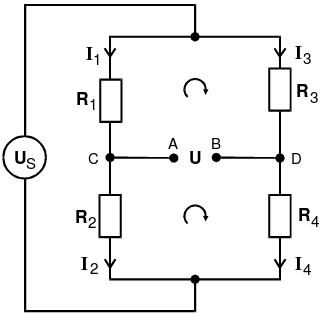
\includegraphics[width=7.50cm, height=6cm]{V302_Brückenschaltung.png}
  \caption{Grundlegende Struktur einer Brückenschaltung\cite{anleitung01}}
  \label{fig:Brückenschaltung}
\end{figure}

Es wird ausgenutzt, dass zwischen zwei getrennten stromdurchflossenen
Leitern eine Potentialdifferenz besteht, die durch die \emph{Kirchhoffschen Gesetze}
bestimmt werden kann.\\\\

1.\emph{Kirchhoffsches Gesetz} (Knotenregel):\\
Die Summe aller in ein Knoten eingehenden Ströme ist gleich der Summe, der aus
einem Knoten herausfließenden Ströme. Diese Gleichung ergibt sich aus der
Ladungserhaltung.

\begin{equation}
  \label{eqn:Kirchhoff1}
  \sum\ua{k} I\ua{k} = 0
\end{equation}

2.\emph{Kirchhoffsche Gesetz} (Maschenregel):\\
Die Summe aller Spannungen in einer Masche ist gleich Null.
Dieses Gesetzt entstammt aus der Energieerhaltung.

\begin{equation}
  \label{eqn:Krichhoff2}
  \sum\ua{k}U\ua{k} = \sum\ua{k}I\ua{k}R\ua{k}
\end{equation}

Der Zusammenhang zwischen der Brückenspannung $U$ und der Speisespannung $U\ua{S}$
ist durch folgenden Zusammenhang gegeben.

\begin{equation}
  \label{eqn:BrückenUndSpeisespannung}
  U\ua{Br} = \frac{R\ua{2}R\ua{3} - R\ua{1}R\ua{4}}{(R\ua{3} + R\ua{4})(Rua{1} + R\ua{2})}U\ua{S}
\end{equation}

Eine Brücke wird als abgeglichen bezeichnet, wenn die Brückenspannung $U\ua{Br}$ verschwindet.
Dies ist gerade der fall, wenn

\begin{equation}
  \label{eqn:abgleichbed}
  R\ua{1}R\ua{4} = R\ua{2}R\ua{3}
\end{equation}

erfüllt ist.
Diese Bedingung ist unabhängig von der Speisespannung $U\ua{S}$
und gilt somit für jede beliebige Speisespannung.

\subsection{Komplexe Wechselstromwiderstände}

Komplexe Wechselstromwiderstände treten auf, wenn Kondensatoren und oder Induktivitäten
in einer Schaltung verbaut sind. Für die Bauteile ergibt sich

\begin{equation*}
  Z\ua{R} = R, \qquad Z\ua{C} = \frac{1}{i\omega C}, \qquad Z\ua{L} = i\omega L.
\end{equation*}

Eine Komplexe Zahl besteht allgemein aus einem Realteil $X$ und einem Imaginärteil
$Y$. Also ist $Z$ insgesamt $Z = X + iY$.

Dabei ist $i$ die imaginäre Zahl und $\omega$ die Kreisfrequenz, mit der die
Spannung wechselt. Damit die Abgleichbedingung \eqref{eqn:abgleichbed} für die
Brückenschaltung für komplexe Widerstände erfüllt ist müssen der Realteil und der
Imaginärteil des Gesamtwiderstandes einzeln verschwinden. Somit ergibt sich

\begin{align}
  X\ua{1}X\ua{4} - Y\ua{1}Y\ua{4} &= X\ua{2}X\ua{3} - Y\ua{2}Y\ua{3}\label{eqn:RealteilAbgleichbed}\\
  X\ua{1}Y\ua{4} + X\ua{4}Y\ua{1} &= X\ua{2}Y\ua{3} + x\ua{3}Y\ua{3}\label{enq:ImaginärteilAbgleichbed}.
\end{align}

Dabei ist $X\ua{i}$ der Realteil und $Y\ua{i}$ der Imaginärteil.

\section{Versuchsaufbau}

In dem Versuch wurden verschiedene Brückenschaltungen verwendet. In dem folgendem
Abschnitt werden die verwendeten Schaltungen erläutert und die dazugehörigen
Formeln angegeben.

\subsection{Wheatstonesche Brücke}

Die Wheatstonesche Brücke wird für die Widerstandsmessung eines unbekannten
Widerstandes verwendet. In der Schaltung werden ausschließlich ohmsche Widerstände
verwendet.

\FloatBarrier
\begin{figure}
  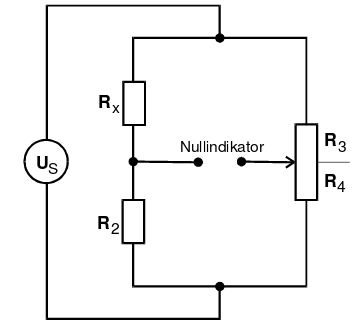
\includegraphics[width=7.50cm, height=6cm]{V302_Wheatstone.png}
  \caption{Schaltungsskizze einer Wheatstonsche Brückenchaltung\cite{anleitung01}}
  \label{fig:Wheatstone}
\end{figure}
\FloatBarrier

Der unbekannte Widerstand lässt sich mit Hilfe von \eqref{eqn:Kirchhoff1} und
\eqref{eqn:Krichhoff2} ermitteln. Es ergibt sich
\begin{equation}
  \label{eqn:Wheatstone}
  R\ua{x} = R\ua{2}\frac{R\ua{3}}{R\ua{4}}.
\end{equation}

Dabei werden $R\ua{3}$ und $R\ua{4}$so eingestellt, dass die Brücke nach
der Bedingung \eqref{eqn:abgleichbed} abgeglichen ist.

\subsection{Kapazitätsmessbrücke}

Ein idealer Kondensator kann durch ergänzen eines ohmschen Widerstandes zu einem
realen Kondensator umgewandelt werden. Ein realer Kondensator ist verlustbehaftet.
Diese Eigenschaft wird von dem ergänzten ohmschen Widerstand übernommen.
Mit Hilfe einer Kapazitätsmessbrücke kann die Kapazität und der Widerstand eines
realen Kondensators bestimmt werde.
Dafür wird der in Abb. \ref{fig:Kapazitätsmessbrücke} Aufbau verwendet.

\begin{figure}
  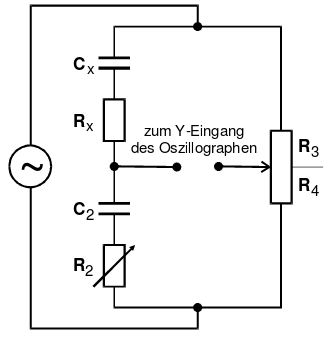
\includegraphics[width=7.50cm, height=6cm]{V302_Kapazitätsmessbrücke.png}
  \caption{Schaltungsskizze einer Kapazitätsmessbrücke\cite{anleitung01}}
  \label{fig:Kapazitätsmessbrücke}
\end{figure}

Über die Knoten- und Maschenregel ergeben sich für die unbekannten Größen
$R\ua{x}$ und $C\ua{x}$ folgende Gleichungen.

\begin{align}
  R\ua{x} &= R\ua{2}\frac{R\ua{3}}{R\ua{4}}\label{KapazitätsmessbrückeRx}\\
  C\ua{x} &= C\ua{2}\frac{R\ua{4}}{R\ua{3}}\label{KapazitätsmessbrückeLx}
\end{align}

\subsection{Induktivitätsmessbrücke}

Die Induktivitätsmessbrücke ist der Kapazitätsmessbrücke sehr ähnlich, nur anstelle
des zu bestimmenden Kondensators die zu vermessende Spule eingebaut wird.
Ebenso ist die ideal Spule mit einem ohmschen Widerstand zu versehen, sodass
die sie das Verhalten einer realen Spule beschreibt.
\begin{figure}
  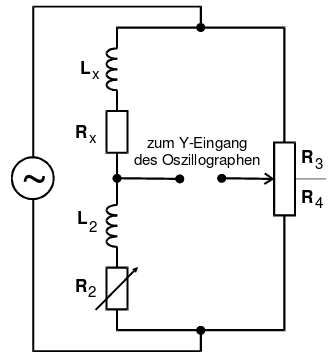
\includegraphics[width=7.50cm, height=6cm]{V302_Induktivitätsmessbrücke}
  \caption{Schaltungsskizze einer Induktivitätsmessbrücke\cite{anleitung01}}
  \label{fig:Induktivitätsmessbrücke}
\end{figure}

Durch die Komplexen Abgleichbedingungen \eqref{eqn:RealteilAbgleichbed} und
\eqref{enq:ImaginärteilAbgleichbed} ergeben sich

\begin{align}
  R\ua{x} &= R\ua{2}\frac{R\ua{3}}{R\ua{4}}\label{InduktivitätmessbrückeRx}\\
  L\ua{x} &= L\ua{2}\frac{R\ua{3}}{R\ua{4}}.\label{InduktivitätmessbrückeLx}
\end{align}

Die Induktivität und der Widerstand von einer realen Spule ist mit der
Induktivitätsmessbrücke schwierig zu vermessen. Der Wirkanteil sollte
möglichst alleine durch $R\ua{2}$ realisiert werden und $L\ua{2}$ sollte
eine möglichst hohe Effizienz haben, damit $L\ua{x}$ und $R\ua{x}$ präzise vermessen
werden können. Dies ist experimentell schwierig umzusetzen.
Deshalb wird für die Messung von Induktivitäten die Maxwell-Brücke verwendet.

\subsection{Maxwell-Brücke}

Bei der Maxwell-Brücke wird parallel zum vierten ohmsche Widerstand $R\ua{4}$
eine Kondensator mit der Kapazität $C\ua{4}$ geschaltet. Die Schaltung ist in
Abb. \ref{fig:Maxwell-Brücke} skizziert.

\begin{figure}
  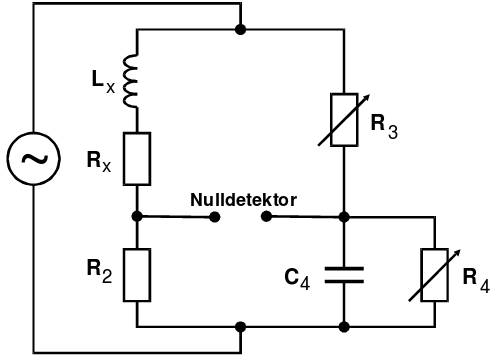
\includegraphics[width=7.50cm, height=6cm]{V302_MaxwellBrücke.png}
  \caption{Schaltungsskizze einer Maxwell-Brücke\cite{anleitung01}}
  \label{fig:Maxwell-Brücke}
\end{figure}

Durch die Komplexen Abgleichbedingungen \eqref{eqn:RealteilAbgleichbed} und
\eqref{enq:ImaginärteilAbgleichbed} ergeben sich

\begin{align}
  R\ua{x} &= \frac{R\ua{2}R\ua{3}}{R\ua{4}}\label{eqn:Maxwell_Rx}\\
  L\ua{x} &= R\ua{2}R\ua{3}C\ua{4}.\label{eqn:Maxwell_Lx}
\end{align}

Die Regelwiderstände $R\ua{3}$ und $R\ua{4}$ werden als Abgleichelemente verwendet
und der Kondensator sollte für eine präzise Messung möglichst verlustarm sein.

\subsection{Wien-Robinson-Brücke}
Die Wien-Robinson-Brücke ist eine frequenzabhängige Brückenschaltung. Der Zusammenhang
zwischen der Brückenspannung und der Speisespannung kann über die Formel
\eqref{eqn:BrückenUndSpeisespannung} berechnet werden.

\begin{equation}
  \label{eqn:Wien-Robinson-Brücke}
  \left|\frac{U\ua{Br}}{U\ua{S}}\right|^2 = \frac{\left(\omega^2R^2C^2 - 1\right)^2}{
  9\left[\left(1 - \omega^2R^2C^2\right)^2 + 9\omega^2R^2C^2\right]}
\end{equation}

Die Brückenspannung verschwindet für die Frequenz $\omega\ua{0} = \frac{1}{RC}$.
Somit wird die Frequenz $\omega\ua{0}$ gefiltert und alle Schwingungen mit
der Frequenz $\omega\ua{0}$ werden nicht durch diese Brückenschaltung durchgelassen.
Schwingungen mit einer Frequenz nahe von $\omega\ua{0}$ werden stark abgeschwächt.

\begin{figure}
  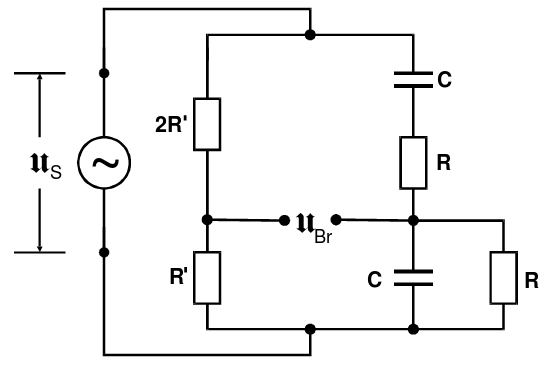
\includegraphics[width=7.50cm, height=6cm]{V302_Wien-Robinson_Brücke.png}
  \caption{Schatungsskizze einer Wien-Robinson-Brücke\cite{anleitung01}}
  \label{fig:Wien-Robinson-Brücke}
\end{figure}

\subsection{Klirrfaktor}

In dem Versuch soll der Klirrfaktor des verwendeten Sinusgenerator bestimmt werden.
Der Klirrfaktor ist eine Zeichen der Güte eines Generators und beschreibt die
Anteile der Oberwellen im Verhältnis zu der Grundwelle.
Der Klirrfaktor kann mit Hilfe der Wien-Robinson-Brücke (Abb.\ref{fig:Wien-Robinson-Brücke})
ermittelt werden. Dafür stellt man die Widerstände so ein, dass die Brückenspannung
minimal ist. An diesem Minimun ist die Frequenz $\omega\ua{0}$ erreicht, bei dem
nur noch die Oberwellen des Sinusgenerators durch die Schaltungen gelassen werden.\\
Der Klirrfaktor ist definiert als:

\begin{equation}
  \label{eqn:Klirrfaktor}
  k := \frac{\sqrt{U\ua{2}^2} + U\ua{3}^2 + ... }{U\ua{1}}.
\end{equation}

Dabei ist $U\ua{1}$ die Amplitude der Grundwelle und $U\ua{i}$ die Amplitude der
i-ten Oberwelle. Zur vereinfachten Rechnung wird hierbei lediglich $U\ua{2}$
berücksichtigt.

\newpage
\printbibliography

\end{document}
